\documentclass[a4paper]{report}
\usepackage[utf8]{inputenc}
\usepackage[T1]{fontenc}
\usepackage{RJournal}
\usepackage{amsmath,amssymb,array}
\usepackage{booktabs}


% tightlist command for lists without linebreak
\providecommand{\tightlist}{%
  \setlength{\itemsep}{0pt}\setlength{\parskip}{0pt}}

\usepackage{longtable}

% Always define CSL refs as bib entries are contained in separate doc
% Pandoc citation processing
\newlength{\cslhangindent}
\setlength{\cslhangindent}{1.5em}
\newlength{\csllabelwidth}
\setlength{\csllabelwidth}{3em}
\newlength{\cslentryspacingunit} % times entry-spacing
\setlength{\cslentryspacingunit}{\parskip}
% for Pandoc 2.8 to 2.10.1
\newenvironment{cslreferences}%
  {}%
  {\par}
% For Pandoc 2.11+
\newenvironment{CSLReferences}[2] % #1 hanging-ident, #2 entry spacing
 {% don't indent paragraphs
  \setlength{\parindent}{0pt}
  % turn on hanging indent if param 1 is 1
  \ifodd #1
  \let\oldpar\par
  \def\par{\hangindent=\cslhangindent\oldpar}
  \fi
  % set entry spacing
  \setlength{\parskip}{#2\cslentryspacingunit}
 }%
 {}
\usepackage{calc}
\newcommand{\CSLBlock}[1]{#1\hfill\break}
\newcommand{\CSLLeftMargin}[1]{\parbox[t]{\csllabelwidth}{#1}}
\newcommand{\CSLRightInline}[1]{\parbox[t]{\linewidth - \csllabelwidth}{#1}\break}
\newcommand{\CSLIndent}[1]{\hspace{\cslhangindent}#1}


\usepackage[labelformat=simple]{subcaption}
\renewcommand\thesubfigure{(\alph{subfigure})}
\usepackage{tikz,enumitem}
\usetikzlibrary{positioning, arrows.meta, shapes.geometric}
\tikzset{%
  semithick,
  >={Stealth[width=2mm, length=2.75mm]},
  obs/.style = {name = #1, circle, draw, inner sep = 5pt, label = center:\(\scriptstyle#1\)},
  fixed/.style = {name = #1, regular polygon, regular polygon sides = 4, draw, inner sep = 3pt, label = center:\(#1\)},
  lat/.style 2 args = {name = #1, circle, draw, dashed, inner sep = 5pt, label = center:\(\scriptstyle#2\)},
}
%\newtheorem{lemma}{Lemma}
\newcommand\independent{\protect\mathpalette{\protect\independenT}{\perp}}
\def\independenT#1#2{\mathrel{\rlap{\(#1#2\)}\mkern2mu{#1#2}}}
\newcommand{\+}[1]{\ensuremath{\mathbf{#1}}}
\newcommand{\doo}{\textrm{do}}


\begin{document}


%% do not edit, for illustration only
\sectionhead{Contributed research article}
\volume{15}
\volnumber{3}
\year{2023}
\month{September}
\setcounter{page}{191}

\begin{article}
  % !TeX root = RJwrapper.tex
\title{Two-Stage Sampling Design and Sample Selection with the R Package R2BEAT}


\author{by Giulio Barcaroli, Andrea Fasulo, Alessio Guandalini, and Marco D. Terribili}

\maketitle

\abstract{%
R2BEAT (``R `to' Bethel Extended Allocation for Two-stage sampling'')
is an R package for the optimal allocation of a sample. Its
peculiarity lies in properly addressing allocation problems for
two-stage and complex sampling designs with multi-domain and
multi-purpose aims. This is common in many official and non-official
statistical surveys, therefore R2BEAT could become an essential tool
for planning a sample survey. The functions implemented in R2BEAT
allow the use of different workflows, depending on the available
information on one or more interest variables. The package covers all
the phases, from the optimization of the sample to the selection of
the Primary and Secondary Stage Units. Furthermore, it provides
several outputs for evaluating the allocation results.
}

\section{Introduction}
Sample surveys carried out by National Statistical Institutes (NSIs) and by other institutions have multi-domain and multi-purpose objectives, so they have to provide accurate estimates for different parameters and different domains (i.e. geographical areas such as national, regional, and more).

Surveys have budgetary and logistical constraints, so they must be carefully planned to provide high-quality estimates for parameters of interest.
In this context, several decisions need to be made, such as sample size, stratification, allocation of sampling units among the strata and multiple-stage.

These decisions may not be trivial and can strongly affect all the following steps of the survey and, moreover, the quality of the results.
This justifies the care and attention typically given in the literature.
A seminal work in this perspective is that of \citet{kish1965survey} and, later, different approaches have been proposed for defining optimal sampling strategies, i.e. maximizing data quality within budgetary constraints \citep[see among the others][]{cochran1977sampling}. 

%Several software and packages have been implemented with the aim of providing a tool and helping researchers in defining the optimal sampling strategy.

The proposed package, R2BEAT (standing for {R} "to" Bethel Extended Allocation for Two-stage), fits into this context and fills a gap within the range of statistical software concerning sample size allocation, thereby introducing an improvement into the R community. 

There are several {R} packages for allocating a stratified sample, such as {surveyplanning} \citep{surveyplanning}, {PracTools} \citep{practools}, {samplesize4surveys} \citep{Rojas:2020}, {optimStrat} \citep{optimstrat} and {SamplingStrata} \citep{barcaroli2014samplingstrata}.
But R2BEAT, extending the methodology implemented in the Italian National Institute of Statistic's open-source software called {Mauss-R} ("Multivariate Allocation of Units in Sampling Surveys") \citep{maussr}, enables us also to compute the optimal allocation among strata for two-stage and complex sampling design considering both multivariate and multi-domain cases.

In the following section the methodological aspects, underlying the package and its functions, will be presented in detail: the optimal allocation of the sample and its selection will be illustrated. 
In the third section will be shown how to prepare, organize and check the input data needed by the package for allocating the whole sample size among strata and finally select the units. 
A case study on a synthetic dataset will be used as an example to test the package functions, and also for a comparison to the other two packages handling two-stage sample design ({PracTools} and {samplesize4surveys}). 
Finally, the concluding remarks will point out that R2BEAT can allocate the sample more efficiently than the other available 
multistage allocation software, while also being strongly flexible, generalizable, and integrated with software that manages all the different phases of the statistical data production process.


\section{Methodological aspects}
\subsection{The optimal allocation}
Let us consider a population $U$ of size $N$ ($k=1, \dots, N$) partitioned in $H$ subgroups, $U_h$ $(h = 1, \dots, H)$, called strata.
Hence, each stratum contains $N_h$ elements, where $N_h$ is assumed to be known such that $\sum_{h=1}^{H} N_h = N$. 

The strata can be defined in different ways on the basis of one or more qualitative variables known for all the units in the population.
%In official statistics, the strata are usually defined according to the lower level at which the estimates are required.

Then, we assume, at least for the moment, to be interested in investigating the mean of just one $y$ variable in the population $U$,
\begin{eqnarray}
	\label{eq:meanPOP}
	\mu_{y} = \frac{\sum_{k \in \ U} y_k}{N}
\end{eqnarray}
where $y_k$ is the value of the $y$ variable observed on the $k$-th unit in the population $U$.
The $y$ variable could be a quantitative variable or dichotomous, that is $y \in \left\lbrace 0, 1 \right\rbrace$.
Please note that, even when $y$ is a dichotomous variable, expression~\eqref{eq:meanPOP} holds and $\mu_{y}$ is equal to the proportion of units in the population for which $y=1$.

Furthermore, assume we want to estimate $\mu_{y}$ through a probabilistic sample $s$ of size $n$ with the estimator
\begin{eqnarray}
	\label{eq:HT}
	\hat{\bar{Y}} = \frac{\hat{Y}_{HT}}{N} = \frac{\sum_{k \in s} y_k \ d_k}{N}
\end{eqnarray}
where $\hat{Y}_{HT}$ is the Horvitz-Thompson estimator for the total \citep{horvitz1952generalization} in which $d_k$ is the design weight usually equal to the inverse of the first order inclusion probability.
%The sampling variance estimator of $\hat{\bar{Y}}$ is given by
%\begin{eqnarray}
%\label{eq:varHT}
%\widehat{\text{var}} \left(\hat{\bar{Y}} \right) = \frac{1}{N^2} \sum_{k \in s} \sum_{\ell \in s} \frac{\pi_{k\ell}- \pi_k \ \pi_\ell}{\pi_{k\ell}} \frac{y_k}{\pi_k} \frac{y_\ell}{\pi_\ell} 
%\end{eqnarray}
%while the relative error is
%\begin{eqnarray}
%\label{eq:CVHT}
%\widehat{\text{CV}} \left(\hat{\bar{Y}} \right) = \frac{\sqrt{\hat{\text{var}} \left(\hat{\bar{Y}} \right)}}{\hat{\bar{Y}}}. 
%\end{eqnarray}

The sample size of a survey, $n$, is usually exogenous information, dictated by budget and, sometimes, by logistic constraints associated with the unit $k$ in the sample.
Then, in practice, the problem comes down to the allocation of the $n$ units in the $H$ strata, such that $\sum_{h=1}^H n_h=n$.

Therefore, let us define 
\begin{eqnarray}
	\label{eq:meanPOPstr}
	\mu_{hy} = \frac{\sum_{U} y_k \ \boldsymbol{1}_h}{N_h}
\end{eqnarray}
the mean of the $y$ in each stratum where $\boldsymbol{1}_h$ is the membership indicator for the unit $k$ in the stratum $h$.


In the same way, expression~\eqref{eq:HT} can be easily adapted for estimating $\mu_{hy}$, that is
\begin{eqnarray}
	\label{eq:HTh}
	\hat{\bar{Y}}_h = \frac{\hat{Y}_{HT,h}}{N_h} = \frac{\sum_{k \in s_h} y_k \ d_k}{N_h},
%Unità N con k da 1 a N
\end{eqnarray}
where $s_h$ is the sample in the stratum $h$.
The sampling variance estimator of $\hat{\bar{Y}}_h$ is given by
\begin{eqnarray}
	\label{eq:varHTh}
	\widehat{\text{var}} \left(\hat{\bar{Y}}_h \right) =
	\frac{1}{n_h - 1} \left(\frac{1}{n_h} - \frac{1}{N_h} \right)
	\sum_{k \in h} (y_{hk} - \bar{y}_h)^2,
	%	\widehat{\text{var}} \left(\hat{\bar{Y}}_h \right) = \frac{1}{N^2} \sum_{k \in s_h} \sum_{\ell \in s_h} \frac{\pi_{k\ell}- \pi_k \ \pi_\ell}{\pi_{k\ell}} \frac{y_k}{\pi_k} \frac{y_\ell}{\pi_\ell}.
\end{eqnarray}
where $\bar{y}_h$ is the sample mean of the variable $y$ in the stratum $h$. 

The mean of $y$ in \eqref{eq:meanPOP} can be written also as 
$\mu_{y}= \sum_{h=1}^H \left({N_h} / {N} \right) \mu_{hy}$
and, consequently, $\hat{\bar{Y}}$ in \eqref{eq:HT} as
$\hat{\bar{Y}} = \sum_{h=1}^H \left( {N_h} / {N} \right) \hat{\bar{Y}}_h$.
Therefore, the sampling variance estimator for $\hat{\bar{Y}}$ is
$\widehat{\text{var}} \left( \hat{\bar{Y}} \right) = \sum_{h=1}^H \left({N_h} / {N} \right)^2 \widehat{\text{var}} \left(\hat{\bar{Y}}_h \right)$.

When there is no information on $y$, the sample size to be allocated to each stratum, $n_h$, can be assigned by performing uniform or proportional allocation.

Uniform allocation assigns an equal number of sampling units to each stratum, that is 
%\begin{eqnarray*}
$
n_h^{UNIF}={n}/{H}.
$
%\end{eqnarray*}

More often, we want the sample size assigned to strata in the sample to be proportional to the sizes of the strata in the population, that is
%\begin{eqnarray*}
$
n_h^{PROP}=n \ \left( {N_h} / {N} \right)
$
%\end{eqnarray*}
where $N_h/N$ is the weight of the stratum in the population with $\sum_{h=1}^H N_h/N=1$.
If the size is the same for all strata ($N_1=\dots=N_h=\dots=N_H=N/H$), $n_h^{PROP}$ comes down to $n_h^{UNIF}$. 

When there is information in the population strata on $y$ and in particular on its variance, $S_{yh}^2$, a more favorable allocation can be performed.
Alternatively, it is possible to consider also a proxy variable highly correlated with $y$.
In this case, \cite{tschprow1923optimal} demonstrated that the optimal allocation can be obtained by 
\begin{eqnarray*}
	n_h^{OPT}=n \frac{\frac{N_h}{N} \ \sqrt{S_{yh}^2}}{\sum_{h=1}^H \frac{N_h}{N} \ \sqrt{S_{yh}^2}}  \end{eqnarray*}
However, this result, also published by 
\citeauthor{neyman1934optimal} 
(\citeyear{neyman1934optimal}), is more often referred to as Neyman's allocation.
The rationale behind the optimal allocation is that strata with more weight and in which $y$ has much more variability need many more observations to reach better estimates. 
If the variance is the same in all the strata ($S_1^2=\dots=S_h^2=\dots=S_H^2$), $n_h^{OPT}$ comes down to $n_h^{PROP}$. 

The computation of the population variance is a crucial point in the optimal allocation.
A distinction between the types of variables and the sources from which they can be obtained is needed.
When $y$ is a dichotomous variable available from a population register, its population variance can be computed as
\begin{eqnarray}
	\label{S2dicho}
	S_{yh}^2 = p_h \times (1 - p_h)
\end{eqnarray}
where $p_h$ is the proportion of units with $y=1$ in the population strata. 
In the case of a quantitative variable, $S_{yh}^2$ is equal to 
%\begin{eqnarray*}
$
\label{S2quant_register}
S_{yh}^2  = \left[ {\sum_{k \in U_h} \left( y_k - \mu_{yh} \right)^2} \right] / {N_h}.
$
%\end{eqnarray*}

When there is no population register, information on the variability can be obtained from a sample survey or a pilot survey which has previously been carried out. 
Let us assume to have collected the $y$ variable, or at least its proxy variable, on a sample $s^*$. 
Then, (\ref{S2dicho}) can be computed just by replacing $p_h$ with 
\begin{eqnarray}
	\label{eq:estp}
	\hat{p}_h = \frac{\sum_{k \in s_h^*} y_k \ w_k}{\sum_{k \in s_h^*} w_k},     
\end{eqnarray}
that is the related estimate for each stratum obtained from the sample $s^*$.
In \eqref{eq:estp} $w_k$ is the sampling weight associated with the unit $k$ in the sample $s^*$. 

Instead, when $y$ is a quantitative variable,
$\label{S2quant_survey} 
S_{yh}^2  =  \hat{M}_h^2 - \hat{\bar{Y}}_h^{2}$
where 
$\hat{M}_h^2 = \left( {\sum_{k \in s_h^*} y_{k}^2 \ w_k} \right) / {N}$ and $\hat{\bar{Y}}_i = \left( {\sum_{k \in s_h^*} y_{k} \ w_k} \right) / {N}$
are the quadratic mean and the arithmetic mean estimated on the sample $s^*$ in the $h$-th stratum, respectively. 

%Sometimes, collecting data on units belonging to different strata can have different costs for the difficulties in reaching them (e.g. strata are altitude zone) or the need of using different data collection modes.
%Therefore, it is advisable to define the allocation by taking into account also the unit cost and the budget constraints.

%The global cost of the survey can be defined as
%\begin{eqnarray*}
%	C=c_0 + \sum_{h=1}^L n_h \ c_h,
%\end{eqnarray*}
%where $c_0$ is the fixed cost (not dependent on the sample size) and $c_h$ is the unit cost for collecting data on one unit belonging to stratum $h$.
%Then, the optimal allocation under budget constraints is given by
%\begin{eqnarray*}
%	n_h^{\bar{OPT}}=(C-c_0) \frac{\frac{\frac{N_h}{N} \ \sqrt{S_{yh}^2}}{\sqrt{c_h}}}{\sum_{h=1}^L \frac{N_h}{N} \ \sqrt{S_{yh}^2} \sqrt{c_h}}.
%\end{eqnarray*}
%If $c_1=\dots=c_h=\dots=c_L=1$ and $c_0=0$, the global cost amounts to the sample size ($C=n$).

The optimal allocation for just one $y$ variable is of little practical use unless the various variables under study are highly correlated. 
This is because an allocation that is optimal for one characteristic is generally far from being optimal for others.

Therefore, several works have been devoted to solving the problem when more than one variable of interest has to be measured on each sampled unit.
All the contributions can be classified into two main approaches: the ``average variance" and convex programming.

The methods under the ``average variance" approach consist of defining a weight for each variable to consider, computing a weighted average of the stratum variance and finding the optimal allocation using the ``average variance" which results.
They are computationally simple, intuitive and can be solved under fixed cost assumption.
However, the choice of the weights is completely arbitrary and the optimal properties are not clear \citep[see, e.g.,][for more details]{kish1976optima}.

Instead, the other approach includes methods that use convex programming to find the minimum cost allocation, satisfying the fixed constraints regarding the variances of all the sampling variables.     
The obtained allocation is actually optimal, but sometimes it can exceed the budgetary constraints.
%\citep[see, e.g.,][for more details]{dalenius1957sampling,yates1960sampling,kokan1963optimum,hartley1965multiple,kokan1967optimum,chatterjee1968multivariate,chatterjee1972study,huddleston1970optimal,bethel1985optimum,chromy1987design,falorsi1998principi,stokes2004using,choudhry2012sample,kozak2007modern,kozak2008stratified}. 

The most important method in the convex programming approach is the Bethel algorithm \citep{bethel1989sample} which extends the Neyman allocation to the multivariate case, providing the optimal allocation in the strata, in terms of surveying cost, according to a set of variables observed in a multidomain context.

In particular, when we are interested in investigating the mean of more than one $y$ variable (quantitative or dichotomous), namely $y_1, \dots, y_i, \dots, y_I$, the optimal allocation problem reduces, in practice, to a minimum optimization problem of a convex function under a set of linear constraints
\begin{eqnarray}
	\label{eq:optprob}
	\left\lbrace
	\begin{array}{l}
		C = \text{min} \\
		\widehat{CV} \left(\hat{\bar{Y}}_{i,h}\right) \leq 
		\delta \left(\hat{\bar{Y}}_{i,h} \right)
		\hspace{0.5cm} \begin{array}{c}
			i = 1, \dots, I \\
			h = 1, \dots, H 
		\end{array}
	\end{array}
	\right.
\end{eqnarray}
where $C$ is the global cost of the survey to be minimized and $\hat{CV} \left(\hat{\bar{Y}}_{i,h}\right)$ is the estimate of the relative error. 
The estimate of the relative error,
\begin{eqnarray}
	\label{eq:CVHTh}
	\widehat{CV} \left(\hat{\bar{Y}}_{i,h} \right) = \frac{\sqrt{\widehat{\text{var}} \left(\hat{\bar{Y}}_{i,h} \right)}}{\hat{\bar{Y}}_{i,h}}, 
\end{eqnarray}
is the ratio between the estimate of the sampling variance for the mean estimator of $y_i$ variable ($i=1, \dots, I$) in  the stratum $h$ given by expression~\eqref{eq:varHTh} and the related estimate.
In this case, $\widehat{CV} \left(\hat{\bar{Y}}_{i,h}\right)$ is called
expected error and it must be less than or equal to the precision constraints defined by the user or by regulation, $\delta \left(\hat{\bar{Y}}_{i,h} \right)$.

\cite{bethel1989sample} demonstrates that the solution to this optimization problem exists and can be obtained through an algorithm that applies the Lagrange multipliers method.
The solution is a real number, so it must be rounded to provide an integer stratum sample size.
The rounding clearly causes some deviations from the solution that, however, do not affect its optimality \citep{cochran1977sampling}.
%The Bethel algorithm is very similar to the Chromy algorithm \citep{chromy1987design}.
%However, it is preferable because, even if the Chromy algorithm is simpler, there is no proof that it converges if a solution exists.

This framework also works in the case of the multi-domain problem.
Usually, estimates of a survey are disseminated for
the whole population and sub-domains, for instance for geographical areas.
Then, it is useful to define the optimal allocation also taking into account these outcomes of the survey.

Sub-domain estimation is actually a long-established theory 
\citep{SSW:03}. 
Expression~\eqref{eq:meanPOP} can be easily adapted just by introducing the sub-domain membership indicator variable, $\boldsymbol{1}_{k,d}$, which equals 1 for each the unit $k$ in the domain $d$ and 0 otherwise, that is
%\begin{eqnarray*}
$
\label{eq:meanPOP_dom}
\mu_y^d = \left( {\sum_{U_d} y_k \ \boldsymbol{1}_{k,d}} \right) / {N_d}
$
%\end{eqnarray*}
where $N_d$ is the population size in the domain $d$ ($d=1, \dots, D$).
It is important to point out, that domains must be an aggregation of strata and thus should not split strata.
Then, it is sufficient to consider the domain estimates in the minimum optimization problem in \eqref{eq:optprob} and use Bethel's algorithm for deriving the multivariate allocation in the multi-domain case. 

However, in official statistics, especially for household surveys, two-stage sampling designs are usually adopted.
Two-stage sampling is based on a double sampling procedure: one on the primary stage units (PSUs) and another on the second stage units (SSUs).
For instance, in the household survey, the PSUs are the municipalities, which are selected first.
Then, in each selected municipality, a sample of households - the $SSU$ - can be selected.

Two-stage sampling permits more complex sampling strategies and, moreover, it helps in the organization and cost reduction of data collection, because it reduces the interviewer's travels.
However, this economic saving is counterbalanced with a loss of efficiency of the estimates.
In fact, each additional stage of selection usually entails an increase of the sampling variance of the mean estimator.
This increase can be assessed by the design effect ($deff$) that measures how much the sampling variance of $\hat{\bar{Y}}_{i}$, under the adopted sampling design ($des$), is inflated with respect to a simple random sample ($srs$), with the same sample size.
An estimate of the design effect can be given by the expression:
\begin{eqnarray*}
\label{eq:deff}
deff \left( \hat{\bar{Y}}_{i} \right) & = & {\widehat{\text{var}} \left( \hat{\bar{Y}}_{i}\right)_{des}} / {\widehat{\text{var}} \left(\hat{\bar{Y}}_{i}\right)_{srs}}
\end{eqnarray*} 
A rough approximation of the $deff$ can be obtained when the clusters have the same sample size and the same inclusion probability \citep{cicchitelli1992campionamento},
\begin{eqnarray}
	\label{eq:deff1}
	deff \left( \hat{\bar{Y}}_{i} \right) & = & 1+\rho_i \ (b-1)
\end{eqnarray} 
where $b$ is the average cluster (i.e. PSU) size in terms of the final sampling units and $\rho_i$ is the intra-class correlation within the cluster (PSU) for the variable $y_i$ $(i=1, \dots, I)$. 

The intra-class correlation provides a measure of data clustering in PSUs and SSUs. 
In general, if $\rho_i$ is close to 1, the clustering is high and it is convenient to collect only a few units in the cluster. 
Instead, if $\rho_i$ is close to 0, the collection of units from the same cluster does not affect the efficiency of the estimates. 

Also for computing $\rho_i$, we can distinguish whether a population register in which the $y_i$ variables ($i=1,\dots,I$), or at least their proxies, are available or not.
In the former case, a good approximation, given in {\cite{cicchitelli1992campionamento}, is
\begin{eqnarray}
	\label{eq:rho_pop}
	%	\rho_i=1 - \frac{H}{H-1} \frac{D_{w_i}^2}{D_{y_i}^2}  
	\rho_i=1 - \left({D_{w_i}} / {D_{y_i}} \right)  
\end{eqnarray}
where $D_{w_i} = \sum_{h=1}^H \sum_{k=1}^{N_h} \left( y_{i,k} - \mu_{y_{i,h}} \right)^2$ is the deviance within clusters and $D_{y_i} = \sum_{k \in U} \left(y_{i,k} - \mu_{y_i}\right)^2$ is the global deviance of the $y_i$ variable.} 
Remember that $D_{y_i}= D_{w_i} + D_{b_i}$, where
$
D_{b_i} = \sum_{h=1}^H N_h \left(\mu_{yi,h} - \mu \right)^2,
$
is the deviance between clusters.
Therefore, $0 \leq \rho_i \leq 1$. 

Instead, $\rho_i$ can be estimated from a sample with the expression~\eqref{eq:deff1}
\begin{eqnarray}
	\label{eq:rho_est}
	\hat{\rho}_{i} = \left({deff_i - 1} \right) \ \left({b-1} \right).
\end{eqnarray}

Here we consider, directly, a more general expression for the estimate of the $deff$ in terms of the intra-class correlation coefficient.
This expression refers to a typical situation in household surveys where PSUs are assigned to Self-Representing (SR) strata, that is they are included for sure in the sample, or to Not-Self-Representing (NSR) strata, where they are selected by chance.
In practice, this assignment is usually performed by comparing the measure of the size of PSUs to the threshold {\citep[see, e.g.,][]{hansen1953sample}}:
\begin{equation}
	\label{eq:threshold}
	\lambda = \left({\bar{m} \ \Delta} \right) / {f}
\end{equation}
where $\bar{m}$ is the minimum number of SSUs to be interviewed in each selected PSU, $f=n/N$ is the sampling fraction and $\Delta$ is the average dimension of the SSU in terms of elementary survey units.
Then, $\Delta$ must be set to 1 if, for the survey, the selection units are the same as the elementary units (that is, household-household or individuals-individuals), whereas it must be set equal to the average dimension of the households if the elementary units are individuals, while the selection units are the households. 
PSUs with a measure of size exceeding the threshold are identified as SR, while the remaining PSUs are identified as NSR.

Then, the extended expression of $deff$ \citep[see, among others,][]{rojas2016estrategias} is
\begin{equation} 
	\label{eq:deff_ext}
	deff \left(\hat{\bar{Y}}_{i}\right) 
	=  \frac{n}{N^2} \left\lbrace
 \frac{N_{SR}^2}{n_{SR}} \left[ 1 + \left( \rho_{i,SR} \  (b_{SR} - 1 \right) \right] +
	\frac{N_{NSR}^2}{n_{NSR}} \left[ 1 + \left(\rho_{i,NSR} \ (b_{NSR} - 1 \right) \right] \right\rbrace
\end{equation}
where, for $SR$ and $NSR$ strata, 
\begin{itemize}
	\item $N_{SR}$ and $N_{NSR}$ are the population sizes;
	\item $n_{SR}$ and $n_{NSR}$ are the sample sizes;
	\item $\rho_{i,SR}$ and $\rho_{i,NSR}$ are the intra-class correlation coefficients for the variable $i$ ($i=1, \dots, I)$;
	\item $b_{SR}$ and $b_{NSR}$ are the average PSU size in terms of the final sampling units.
\end{itemize} 
Of course, if there are no SR strata, this expression simplifies to Equation \eqref{eq:deff1}. 
The design effect is equal to 1 under the $srs$ design and increases for each additional stage of selection, due to the intra-class correlation coefficient which is, usually, positive.

The intra-class correlation coefficient for NSR can be computed with expression ~\eqref{eq:rho_pop} or \eqref{eq:rho_est} whether population register data are available or not.
It is not necessary to compute the intra-class correlation coefficient for SR strata because just one PSU is selected and the intra-class correlation is 1 by definition.

Therefore, under a two-stage sample design for determining the optimal allocation, the number of PSUs and SSUs must be determined.

A solution which makes iterative use of the Bethel algorithm has been proposed by \cite{falorsi1998principi}.
In fact, at the first iteration, the Bethel algorithm is applied. 
The optimal allocation for a stratified simple sampling design is obtained. 
Then, this allocation is used to update the threshold in \eqref{eq:threshold} and the design effect in \eqref{eq:deff_ext}.
A new design effect is computed and used in turn to inflate the $S_h^2$ (or equivalently $\hat{S}_h^2$).
It is used as input in the next iteration in which the Bethel algorithm is used again.
The obtained allocation is used again to update the threshold and the design effect, and a new allocation is found.
The process is iterated until the difference between two consecutive iterations is lower than a predefined threshold.

\begin{algorithm}[h!]
	\SetAlgoLined
	\SetKwData{Left}{left}
	\SetKwData{This}{this}\SetKwData{Up}{up}
	\SetKwFunction{Union}{Union}
	\SetKwFunction{FindCompress}{FindCompress}
	
	\SetKwInOut{Input}{Input}
	\SetKwInOut{Output}{Output}
	\BlankLine
	\Input{
		\BlankLine
		\begin{itemize}
			\item[a.] precision constraints in terms of CV\;
			\item[b.] information on sampling strata (mean 
			and stdev of target variables, $N$, ...)\;
			\item[c.] information on previous design: 
			$deff$, $effst$, $\rho$\;
			\item[d.] information on PSUs in sampling strata (measure of size)\;
			\item[e.] minimum number of SSUs per PSU\;
		\end{itemize}
	}
	\BlankLine
	\Output{
		\BlankLine
		\begin{itemize}
			\item[a.] for each stratum: number of PSUs and 
			SSUs to be selected\;
			\item[b.] expected CVs for target estimates\;
			\item[c.] sensitivity of the solution\;
		\end{itemize}
	}
	\BlankLine
	\nlset{REM} First iteration\;\label{first}
	\begin{enumerate}
		\item input deff is used to inflate standard 
		deviations of target variables in sampling strata\;
		\item  optimal allocation of SSUs in sampling strata 
		is obtained by applying the Bethel algorithm as if it were a one-stage sampling design\;
		\item  the number of PSUs is determined on the basis 
		of the minimum number of SSUs per PSU\;
		\item  the threshold for determination of self-representing PSUs is calculated\;
		\item new deff is calculated and used to update the standard deviations of target variables in sampling strata\;
	\end{enumerate}
	\nlset{REM} Next iterations\;\label{iterations}
	\While{not convergence} {
		\begin{enumerate}
			\item optimal allocation of SSUs in sampling strata is obtained by applying the Bethel algorithm\;
			\item the number of PSUs is determined on the basis of the minimum number of SSUs per PSU\;
			\item the threshold for determination of self-representing PSUs is calculated\;
			\item new deff is calculated an used to update standard deviations of target variables in sampling strata\;
			\item the iteration stops if \
			\begin{itemize}
				\item[a.] the difference between the 
				sample sizes of two iterations is lower than 5 (default value) \textit{or}
				\item[b.] the maximum of defts (square 
				root of deffs) largest differences is lower than 0.06 (default value) \textit{or}
				\item[c.] the number of iterations is 
				higher than 20 (default value)\;
			\end{itemize}
		\end{enumerate}
	}
	\caption{R2BEAT optimal allocation of PSUs and SSUs in sampling strata}
	\label{algorithm}
\end{algorithm}

However, as pointed out by \cite{waters1987optimal}, different combinations yield the same variance and can satisfy the precision constraints, $\delta \left( \hat{\bar{Y}}_{i,h} \right)$.
The optimal solution strongly depends on the budgetary constraints that limit the $SSU$s and the data collection organization that influences the maximum number of $PSU$s that can be managed.

All this discussion holds when you want to use the $HT$ estimator.   
But, currently, the most applied estimator for the NSIs survey is the calibrated estimator \citep{deville1992calibration}.
The calibrated estimator, through the use of auxiliary variables, usually provides better estimates than $HT$.
The use of a different estimator from the $HT$ can be considered since the allocation phase, by accounting for the estimator effect and following the procedure explained above

An estimate of the estimator effect ($effst$) is given by 
\begin{equation}
	\label{effst}
	effst (\hat{\bar{Y}}_{i}) = \frac{\text{var} \left(\hat{\bar{Y}}_{i} \right)}{\text{var} \left(\hat{\bar{Y}}_{i,_{HT}} \right)}.
\end{equation}
It measures how much the sampling variance of the applied estimator under the adopted design is inflated or deflated with respect to the sampling variance of the $HT$ estimator, on the same sample design.


\subsection{Sample selection}
\label{sec:samplesel}
Once the optimal allocation is defined, the selection of sampling units must be performed.

In the case of a stratified two-stage sampling design two sampling selections need to be done: one for PSUs and one for SSUs.

In each stratum, the PSUs are split into SR and NSR according to a size threshold \eqref{eq:threshold}. 
PSUs with a measure of size exceeding the threshold are identified as SR, included for sure in the sample and each of them constitutes an independent sub-stratum. 
Therefore, the probability that they are included in the sample (inclusion probability,  $\pi_I$) is always equal to 1.

It is possible that that it can happen that no PSU has a measure of size higher than the threshold: this can happen for example when we consider as PSUs the census enumeration areas, whose distribution of the measure of size is about uniform; on the contrary, it is unlikely to happen when we consider municipalities. 

The remaining PSUs, NSR-PSUs, are ordered by their measure of the size and divided into finer strata (\textit{sub-strata}) whose sizes are approximately equal to the threshold multiplied by the number of PSUs to be selected in each stratum.
In this way, sub-strata are composed of PSUs having size as homogeneous as possible. 

The PSUs in each stratum can be selected in different ways.
However, the selection of a fixed number of PSUs per stratum is usually carried out with Sampford's method (unequal probabilities, without replacement, fixed sample size).
%Then, the inclusion probability of the generic $h$-th NSR-PSU, is 
%$
%	\pi_I=\frac{N_h}{m \ M_{hh}}
%$
%where $N_h$ is the measure of size in the sub-stratum $h$-th, $m$ is the number of NSR-PSUs to be selected in the sub-stratum and $M_{hh}$ is the measure of size in the $h$-th PSU in the sub-stratum $h$. 

Finally, the SSUs must be drawn in the selected PSU.
Also in this case the SSU can be selected in different ways.
In most cases, they are selected through a systematic sampling design that shares several properties with the $srs$.
%Then, the inclusion probability for the second stage is equal to
%$
%	\pi_{II}=\frac{n_{hh}}{M_{hh}}
%$
%where $n_{hh}$ is the number of SSUs to be selected in the $h$-th PSU in the %$h$-th sub-stratum.

Then, the design weight for the unit $k$ in the $h$-th strata in the $\ell$-th PSU is equal to the inverse of the product of the first stage and the second stage inclusion probabilities, 
$
d_k = \frac{1}{\pi_{I}} \frac{1}{\pi_{II}}.     
$
The design weights sum up to the population size, $\sum_{k \in s} d_k = N$, and are almost constant in each stratum, which means that the sample is self-weighting.
\begin{algorithm}[h!]
	\SetAlgoLined
	\SetKwData{Left}{left}
	\SetKwData{This}{this}\SetKwData{Up}{up}
	\SetKwFunction{Union}{Union}
	\SetKwFunction{FindCompress}{FindCompress}
	
	\SetKwInOut{Input}{Input}
	\SetKwInOut{Output}{Output}
	\BlankLine
	\Input{
		\BlankLine
		\begin{itemize}
			\item[a.] The output of the allocation step (function 
			\texttt{beat.2st}) (universe of PSUs, measure of PSUs, number of PSUs and SSUs to be selected in each stratum, threshold)\;
		\end{itemize}
	}
	\BlankLine
	\Output{
		\BlankLine
		\begin{itemize} 
			\item[a.] universe of PSUs with stratum, sub-stratum, 
			PSU first order inclusion probability, PSU weight, flag sample, and number of SSUs to be selected in each PSU\;
			\item[b.] sample of PSUs (flag sample=1) with stratum, 
			sub-stratum, PSU first order inclusion probability, PSU weight, number of SSUs to be selected in each PSU\;
			\item[c.] statistics related to the sample of PSUs at 
			stratum level\;
		\end{itemize}
	}
	\BlankLine
	\nlset{REM} creation of \textit{sub-strata} and selection of PSUs\;
	\begin{enumerate} 
		\item in each stratum, PSUs are sorted in descending order 
		according to their measure of size\;
		\item the measure of size of PSUs are compared with the 
		threshold\;
		\item PSUs with a measure of size exceeding the threshold 
		are identified as SR, included for sure in the sample and constitute an independent sub-stratum\;
		\item  the remaining PSUs, NSR-PSUs, are ordered in 
		decreasing way by their measure of size and aggregated into finer strata (\textit{sub-strata})\;
		\item \textit{sub-strata} are created adding PSUs (still 
		in descending order of measure of size) for which the sum of the measure of size of the \textit{sub-strata} is approximately equal to the threshold multiplied by the number of PSUs to be selected in each stratum\;
		\item in each \textit{sub-stratum} a fixed number of PSUs 
		per stratum are usually selected with Sampford's method (unequal probabilities, without replacement, fixed sample size)\;
	\end{enumerate}
	\caption{R2BEAT selection of PSUs}
	\label{algorithm2}
\end{algorithm}

\section{Structure of the package} 
The {R2BEAT} package provides functions for drawing complex sample designs using an optimal allocation also performing  the selection of the PSUs and SSUs.
To install the latest release version of {R2BEAT} from CRAN, type \textbf{install.packages("R2BEAT")}
within {R}. 
The current development version can be downloaded and installed from GitHub by executing \textbf{devtools::install\_github("barcaroli/R2BEAT")}.

%This section provides an introduction to the structure and functions associated with the package while the next section will present examples of its specific use.

The workflow to draw and select a complex sample using {R2BEAT} is: (1) prepare the input data, (2) check the input data,
(3) define the design and obtain the allocation, and (4) select the final sample units.

\subsection{Prepare the input data}
\label{sec:prepinput}
As will be illustrated in detail in the next sub-sections the {R2BEAT} package provides functions to define one-stage stratified sample design (\textbf{beat.1st}) and two-stage stratified sample design (\textbf{beat.2st}). The preparation of the input dataset changes whether the former or the latter sample design will be adopted.

In the case of a multivariate optimal allocation for different domains in a stratified one-stage sample design, the function \textbf{beat.1st} can be used. 
This function requires two inputs, 	
a data frame containing survey strata information (\textbf{stratif}) and a data frame of expected CV for each domain and each variable (\textbf{errors}). No functions to prepare these inputs are provided by the package but is possible to follow the example dataset \textbf{stratif} and \textbf{error} to properly create the input datasets for the function \textbf{beat.1st}.

In the case of a two-stage design, two functions are provided by the package to help in the creation of the input data for the function \textbf{beat.2st}. 
There are two functions because two different scenarios are possible, depending on the initial information available:

1. Only the sampling frame is available, no previous rounds of the survey have been carried out. In this scenario, a strict condition on the information content of the sampling frame must hold: values of the sample target surveys (or of their proxy correlated variables) are available for each unit in the frame. This can be accomplished by considering the previous census, or by using administrative registers. In this scenario, the function \textbf{prepareInputToAllocation1} can be used to create the input dataframes \textbf{stratif}, \textbf{rho}, \textbf{deft}, \textbf{effst}, \textbf{des\_file} and \textbf{psu\_file}.  

2. Together with a sampling frame containing the units of the population of reference, also a previous round of the sampling survey to be planned is available. The \textbf{prepareInputToAllocation2} produces the same outputs of \textbf{prepareInputToAllocation1}, but it requires the design and/or calibrated objects of the previous sample survey, obtained using the {ReGenesees} package \citep{zardetto2015regenesees}. 

The function \textbf{sensitivity\_min\_SSU} allows analyzing the different results in terms of first stage size (number of PSUs) and second stage size (number of SSUs), obtained when varying the values of the minimum number of SSUs to be selected in each PSU.

When using a previous survey, the 'strata' dataframe is automatically obtained by estimating all the 
variables in it, including the 'N', that is the population in strata. Being an estimate, these values
can differ from the ones obtained by the 'des' dataframe (obtained by aggregating PSUs values). It is up to the user to decide if 
PSUs derived N values are more reliable than those obtained by the survey, and, in case, to assign those
to the 'strata' dataframe. To check the coherence between the estimated population in the strata (\textbf{stratif}) and the population calculated by the PSUs dataset (\textbf{des\_file}), the function \textbf{check\_input} is provided to the users. 
This function compares the strata sizes giving information about the differences and replacing the estimated stratum size with the stratum population calculated by the PSUs dataset.

\subsection{Defining the design and determining the allocation} \label{sec:alloc}

The package allows performing the optimal allocation for both one-stage and two-stage stratified sampling.

The first one is implemented within the function \textbf{beat.1st} and computes a multivariate optimal allocation for different domains in a one-stage stratified sample design.
As described in the previous section, in a one-stage stratified sample design there are only two inputs to be provided to \textbf{beat.1st}: the dataframes \textbf{stratif} and \textbf{errors}. Besides these two mandatory inputs, it is also possible to indicate the minimum number of sampling units to be selected in each stratum, by default set equal to 2.

The function \textbf{beat.2st} performs the same multivariate optimal allocation for different domains considering stratified two-stage design. 
Together with the input data \textbf{stratif} and \textbf{errors} other mandatory input are: 

\begin{itemize}
	\item \textbf{des\_file}: dataframe containing a row per each stratum, with information on total population, the values of the \textbf{delta} parameter (equal to the mean number of final SSUs contained in clusters to be selected, for instance, the mean number of individuals in a household), and the minimum number of SSUs to be selected in each PSU;
	\item \textbf{psu\_file}: dataframe containing information on each PSUs (identifier, stratum, measure of size).
	\item \textbf{rho}: dataframe contains a row per each stratum with the intra-class correlation coefficient both for self representing and non-self representing PSUs.
\end{itemize}

Is also possible to provide optional information about:

\begin{itemize}
	\item \textbf{deft\_start}: dataframe containing a row per each stratum with the starting values for the square root of the design effect in the stratum of each variable of interest.
	\item \textbf{effst}: dataframe containing a row per each stratum with the estimator effect for each variable of interest.
\end{itemize}

The functions \textbf{beat.1st} and \textbf{beat.2st} produce lists with respectively 4 and 9 items. 

The \textbf{beat.1st} output contains:
\begin{enumerate}
	\item \textbf{n}: a vector with the optimal sample size for each stratum;
	\item \textbf{file\_strata}: a dataframe corresponding to the input dataframe \textbf{stratif} with the $n$ optimal sample size column added;
	\item \textbf{alloc}: a dataframe with optimal (\textbf{ALLOC}), proportional (\textbf{PROP}), equal (\textbf{EQUAL}) sample size allocation;
	\item \textbf{sensitivity}: a data frame with a summary of planned coefficients of variation (\textbf{Planned CV}), the expected ones under the given optimal allocation (\textbf{Actual CV}), and the sensitivity at 10\% for each domain and each variable. Sensitivity can be a useful tool to help in finding the best allocation, as it provides a hint of the expected sample size variation for a 10\% change in planned CVs.
\end{enumerate}

Together with the previous outputs, the function \textbf{beat.2st} produces also:
\begin{enumerate}
	\item \textbf{iterations}: a dataframe that for each iteration of the Bethel algorithm provides a summary with the number of PSUs (\textbf{PSU\_Total}), distinguished between SR (\textbf{PSU\_SR}) and NSR (\textbf{PSU\_NSR}), plus the number of SSUs;
	\item \textbf{planned}: a dataframe with the planned coefficients of variation for each variable in each domain.
	\item \textbf{expected}: a dataframe with a summary of expected coefficients of variation under the given optimal allocation for each target variable in each domain;
	\item \textbf{deft\_c}: a dataframe with the design effect for each variable in each domain in each iteration. Note that \textbf{DEFT1\_0 - DEFTn\_0} is always equal to 1 if \textbf{deft\_start} is NULL; otherwise it is equal to \textbf{deft\_start}. While \textbf{DEFT1 - DEFTn} are the final design effect related to the given allocation.
	\item \textbf{param\_alloc}: a vector with a resume of all the parameters given for the allocation.
\end{enumerate}

\subsection{Sample units selection} \label{sec:selection}
Once the allocation for the primary and secondary sampling stage units has been defined, it is possible to use two functions for the selection of the final sampling units.

The function \textbf{select\_PSU} allows the users to select the PSUs allocated in each stratum, using the Sampford method, as implemented by the \textbf{UPsampford} function of R package \textbf{sampling} \citep{Rsampling}. 

The input of this function is the output of the \textbf{beat.2st} function.

The output of the function is a list containing the following items:

\begin{enumerate}
	\item \textbf{universe\_PSU}: a dataframe that reports the whole universe of PSUs, with the inner strata formed for the selection;
	\item \textbf{sample\_PSU}: a dataframe containing the selected PSUs, with the indication, for each of them, of how many SSUs must be selected;
	\item \textbf{PSU\_stats}: a table containing summary information on selected PSUs.
\end{enumerate}

In the last step, the selection of a sample of SSUs has to be carried out. The function \textbf{select\_SSU} allows selecting a sample of SSUs from the population frame, based on the SSUs allocated to each selected PSUs. 

The input datasets are two:
\begin{enumerate}
	\item \textbf{df}: the dataframe containing the final sampling units;
	\item \textbf{PSU\_sampled}: the dataframe containing selected PSUs, corresponding to the second item of the output of the \textbf{select\_PSU}function.
\end{enumerate}

The function \textbf{select\_SSU} returns a dataframe containing the  selection of the \textbf{df} dataframe, enriched with information about the first stage inclusion probability, the second stage inclusion probability, the final inclusion probability (the product of the first stage and the second stage inclusion probabilities) and the design weights.

\section{Illustrative examples} \label{sec:example}

To illustrate how to implement workflows making use of \textbf{R2BEAT} functions, we will consider two scenarios, depending on the initial setting:

\begin{enumerate}
	\item only the sampling frame is available, no previous rounds of the survey have been carried out;
	\item together with a sampling frame containing the units of the population of reference, a previous round of the sampling survey to be planned is available;
\end{enumerate}

In both cases, we assume that the sampling frame contains information on the final sampling units, together with the indication of the PSUs to which each unit belongs.
In the first scenario, a stricter condition on the information content of the sampling frame must hold: values of the sample target surveys (or of their proxy correlated variables) must be available for each unit in the frame. This can be accomplished by considering a previous census, or by imputing values using predictive models. 
In the following paragraphs, we will show only a subset of the code necessary to produce the final results, the relevant part of it\footnote{In order to reproduce the processing related to these examples, datasets and R scripts are downloadable from the link  \href{https://zenodo.org/records/10183968}{https://zenodo.org/records/10183968}.}.

\subsection{Scenario 1 workflow}

In this scenario, it is assumed that a sampling frame is available. We consider a frame (\textbf{pop.RData}), containing 2,258,507 units: 

\begin{verbatim}
	'data.frame':   2258507 obs. of  13 variables:
	$ region       : Factor w/ 3 levels "north","center",..: 1 1 1 1 1 1 1 1 1 1 ...
	$ province     : Factor w/ 6 levels "north_1","north_2",..: 1 1 1 1 1 1 1 1 1 1 ...
	$ municipality : num  1 1 1 1 1 1 1 1 1 1 ...
	$ id_hh         : Factor w/ 963018 levels "H1","H10","H100",..: 1 1 1 2 3 3 3 3 1114 1114 ...
	$ id_ind       : int  1 2 3 4 5 6 7 8 9 10 ...
	$ stratum      : Factor w/ 24 levels "1000","2000",..: 12 12 12 12 12 12 12 12 12 12 ...
	$ stratum_label: chr  "north_1_6" "north_1_6" "north_1_6" "north_1_6" ...
	$ sex          : int  1 2 1 2 1 1 2 2 1 1 ...
	$ cl_age       : Factor w/ 8 levels "(0,14]","(14,24]",..: 3 7 8 5 4 6 6 4 4 1 ...
	$ active       : num  1 1 0 1 1 1 1 1 1 0 ...
	$ income_hh    : num  30488 30488 30488 21756 29871 ...
	$ unemployed   : num  0 0 0 0 0 0 0 0 0 0 ...
	$ inactive     : num  0 0 1 0 0 0 0 0 0 1 ...
\end{verbatim}	
covering a (synthetic) population of reference, with basic information (geographical and demographic variables: 
\begin{itemize}
	\item region: the NUTS2 identifier;
	\item province: the NUTS3 identifier;
	\item municipality: identifier of the municipality, that plays the role of the PSU identifier;
	\item id\_hh: the household identifier;
	\item id\_ind: the individual identifier;
	\item stratum and stratum\_label: identifier of the initial strata (provinces);
	\item sex and cl\_age: demographic information on individuals.
\end{itemize}
together with information that is related to the sampling survey we want to design:
\begin{itemize}
	\item \textbf{active}, \textbf{inactive}, \textbf{unemployed}: binary variables indicating the occupation status of the individual; 
	\item \textbf{income\_hh}: household income.
\end{itemize}
We suppose that the values of these variables have been made available by a different source (for instance a census) or by predicting them with a model-based approach. In any case the uncertainty related to these values should be taken into account, by correctly evaluating the anticipated variance related to the models used for the predictions when producing the \textbf{strata} dataset \citep[][p. 59]{Baillargeon+Rivest:2012}.

Anyway, in the following, we will not consider this issue, as we want only to illustrate how it is possible to automatically derive all the inputs required by the next steps.

\subsubsection{Step 1: preparation of the inputs for the optimal sample design}

The function \textbf{prepareInputToAllocation1} allows preparing all the inputs required by the optimal allocation step under this first scenario. 
This function requires the attribution of values to the following parameters:
\textbf{samp\_frame},
\textbf{id\_PSU},
\textbf{id\_SSU}, 
\textbf{strata\_var}, 
\textbf{target\_vars}, 
\textbf{deff\_var}, 
\textbf{domain\_var},
\textbf{delta} (average dimension of the SSU in terms of elementary survey units),
\textbf{minimum} (minimum number of SSUs to be interviewed in each selected PSU).

About the values of these parameters, the choices are almost always driven by the content and structure of the sampling frame, except for \textbf{minimum}. To choose a suitable value for this parameter, the function \textbf{sensitivity\_min\_SSU} allows performing a sensitivity analysis, showing how the first and second stage sample sizes vary by varying their values:

\begin{verbatim}
	> sens_min_SSU <- sensitivity_min_SSU (
	+             samp_frame=pop,
	+             id_PSU="municipality",
	+             id_SSU="id_ind",
	+             strata_var="stratum",
	+             target_vars=c("income_hh","active","inactive","unemployed"),
	+             deff_var="stratum",
	+             domain_var="region",
	+             delta=1,
	+             deff_sugg=1.5,
	+             min=30,
	+             max=80) 
\end{verbatim}

This function calculates 11  different pairs of values for the number of PSUs and SSU as resulting from the allocation step, starting with the value '30' assigned to the parameter \textbf{minimum}, ending with the value '80'.
The results are reported in Figure \ref{PlotMinimum}.


\begin{figure} [h!]
	\centering
	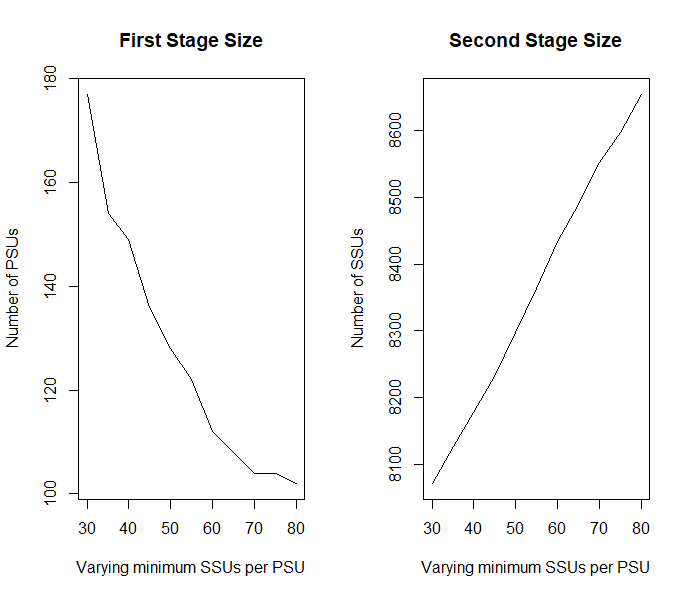
\includegraphics[width=14cm,height=10cm]{Plot_min_SSU.png}
	\caption{Sensitivity analysis for \textbf{minimum} parameter.}
	\label{PlotMinimum}
\end{figure}

On the basis of the results of the sensitivity analysis, we can set the minimum (for instance 50) in the \textbf{prepareInputToAllocation1} function:
\begin{verbatim}
	> inp <- prepareInputToAllocation1(
	+             samp_frame = pop,
	+             id_PSU = "municipality",
	+             id_SSU = "id_ind",
	+             strata_var = "stratum",
	+             target_vars = c("income_hh","active","inactive","unemployed"),
	+             deff_var = "stratum",
	+             domain_var = "region",
	+             delta = delta,     
	+             minimum = 50,
+             deff_sugg = 1.5)
	Computations are being done on population data
	Number of strata:  24
	... of which with only one unit:  0
\end{verbatim}

The output of this function (\textbf{inp}) is a list composed by the following dataframes:
\textbf{strata},
\textbf{deff},
\textbf{effst},
\textbf{rho}, 
\textbf{psu\_file}, 
\textbf{des\_file}.
These will be the inputs for the optimal allocation step (with the exception of the \textbf{deff}), which is produced only for documentation).

\subsubsection{Step 2: optimization of PSUs and SSUs allocation}

It is now possible to execute the optimization step of the sample design. 

First of all, we define the set of precision constraints on the target variables:
\begin{verbatim}
	DOM  CV1  CV2  CV3  CV4
	1 DOM1 0.02 0.03 0.03 0.05
	2 DOM2 0.03 0.06 0.06 0.08
\end{verbatim}
We interpret the values of the CVs in this way: the maximum expected coefficient of variation for the first target variable (\textbf{household income}) is 2\% at the national level and 3\% at the regional level; for \textbf{active} and \textbf{inactive} the expected maximum values of CV is 3\% at the national level and 6\% at the regional level; finally, for \textbf{unemployed} it is 5\% at the national level and 8\% at the regional level.

The optimization step is performed by executing the \textbf{beat.2s} function:

\begin{verbatim}
	> inp1$desfile$MINIMUM <- 50
	> alloc1 <- beat.2st(stratif = inp1$strata, 
	+                   errors = cv, 
	+                   des_file = inp1$des_file, 
	+                   psu_file = inp1$psu_file, 
	+                   rho = inp1$rho, 
	+                   deft_start = NULL,
	+                   effst = inp1$effst, 
	+                   minPSUstrat = 2,
	+                   minnumstrat = 50
	+                   )
	iterations PSU_SR PSU NSR PSU Total  SSU
	1          0      0       0         0 7887
	2          1     31     104       135 8328
	3          2     39     104       143 8318
	4          3     38     104       142 8321
\end{verbatim}

This design is characterized by 142 PSUs (of which 38 self-representative, SR, and 104 non self-representative, NSR) and 8,321 SSUs. 


\subsubsection{Step 3: selection of PSUs and SSUs}

We can now proceed in selecting the PSUs:

\begin{verbatim}
	> sample_1st <- select_PSU(alloc, type="ALLOC", pps=TRUE, plot=TRUE)
	> sample_1st$PSU_stats
	    STRATUM PSU PSU_SR PSU_NSR  SSU SSU_SR SSU_NSR
	1     1000   2      2       0  286    286       0
	2     2000   9      3       6  452    152     300
	3     3000   4      0       4  200      0     200
	...
	23   23000   4      0       4  200      0     200
	24   24000   2      0       2  100      0     100
	25   Total 142     38     104 9421   4221    5200
\end{verbatim}

A discrepancy can be noted between the number of SSUs determined by the allocation step and the one produced by the selection of PSUs. This is because the selection of PSUs controls that the minimum number of SSUs to be allocated in each selected PSU is compliant with the minimum, in our case equal to 50: if not, this minimum is assigned. This is why the total number of SSUs increases from 8,320 to 9,421.

Selected PSUs are contained in the \textbf{sample\_PSU} element of the output list:
\begin{verbatim}
	> head(sample_1st$sample_PSU)
	   PSU_ID STRATUM stratum SR nSR PSU_final_sample_unit Pik weight_1st weight_2st   weight
	1    330    1000  1000-1  1   0                   207   1          1   706.0966 706.0966
	2    309    1000  1000-2  1   0                    72   1          1   706.1806 706.1806
	3     51   10000 10000-0  1   0                   171   1          1   196.8480 196.8480
	4     11   10000 10000-1  1   0                    96   1          1   196.9688 196.9688
	5     40   10000 10000-2  1   0                    79   1          1   197.9494 197.9494
	6     13   10000 10000-3  1   0                    72   1          1   198.3750 198.3750
\end{verbatim}
With this input, we can proceed to select the sample of final units. 
The distribution of PSUs and SSUs in the different strata is reported in Figure \ref{alloca1}. 
\begin{verbatim}
	> PSU_sampled <- sample_1st$sample_PSU
	> samp <- select_SSU(df=pop,
	+                    PSU_code="municipality",
	+                    SSU_code="id_ind",
	+                    PSU_sampled)
	
	--------------------------------
	Total PSUs =  142
	Total SSUs =  9421
	--------------------------------
\end{verbatim}

\begin{figure} [h!]
	\centering
	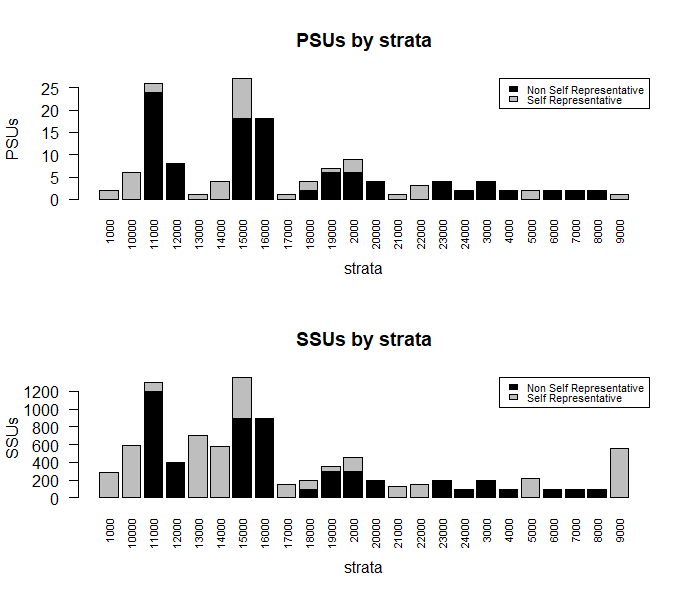
\includegraphics[width=15cm,height=12cm]{allocation1.png}
	\caption{Allocation of PSUs and SSUs (scenario 1).}
	\label{alloca1}
\end{figure}

\subsubsection{Step 4: verify compliance with precision constraints}

The function \textbf{eval\_2stage} allows verifying the compliance of the two-stage sample design to the set of precision constraints, by selecting a given number of different samples (in our case, 500) from the sampling frame, producing the estimates for each sample, and calculating over them the coefficients of variation for each target estimate.

We apply twice the function, first for the national level:
\begin{verbatim}
	> # Domain level = national
	> domain_var <- "one"
	> set.seed(1234)
	> eval11 <- eval_2stage(df,
	+                     PSU_code,
	+                     SSU_code,
	+                     domain_var,
	+                     target_vars,
	+                     sample_1st$sample_PSU,
	+                     nsampl=100, 
	+                     writeFiles=FALSE,
	+                     progress=FALSE) 
	> eval11$coeff_var
     CV1    CV2    CV3    CV4  dom
1 0.0093 0.0099  0.025 0.0356 DOM1
\end{verbatim}
then, at the regional level:
\begin{verbatim}
	> # Domain level = regional
	> domain_var <- "region"
	> set.seed(1234)
	> eval12 <- eval_2stage(df,
	+                     PSU_code,
	+                     SSU_code,
	+                     domain_var,
	+                     target_vars,
	+                     sample_1st$sample_PSU,
	+                     nsampl=100, 
	+                     writeFiles=FALSE,
	+                     progress=FALSE) 
	> eval12$coeff_var
     CV1    CV2    CV3    CV4  dom
1 0.0105 0.0061 0.0224 0.0702 DOM1
2 0.0241 0.0171 0.0452 0.0652 DOM2
3 0.0281 0.0279 0.0533 0.0446 DOM3
\end{verbatim}

We recall that the precision constraints had been set equal to 2\% for the first variable, 3\% for the second and third, and 5\% for the fourth, at national level; and respectively to 3\% and 6\% and 8\% at regional level. We can see that the computed CVs are all compliant.

\subsection{Scenario 2 workflow}
Together with the availability of a sampling frame, containing the same information presented in the previous scenario, we assume also the availability of at least one previous round of the survey.
For sake of simplicity, we assume that the previous round sample is the same selected in scenario 1. We assume also that the values of the four target variables are the observed ones after the data collection. 
Having set the above conditions, the main difference with scenario 1 is that, instead of choosing in a somewhat arbitrarily way the values of the inputs required by the optimal allocation step, we can derive them directly from the collected survey data.

\subsubsection{Step 1: processing and analysis of survey data}
In this step, we proceed to perform the usual phases of calibration and production of the estimates. In doing that, we make use of the R package \textbf{ReGenesees}.

First, we describe the sample design:

\begin{verbatim}
	> ## Sample design description
	> sample$stratum_2 <- as.factor(sample$stratum_2)   # stratum as factor, required by the next function
	> sample.des <- e.svydesign(sample, 
	+                           ids= ~ municipality + id_hh, 
	+                           strata = ~ stratum_2, 
+                           self.rep.str = ~ SR, 
	+                           weights = ~ weight,
	+                           check.data = TRUE)
\end{verbatim}
obtaining the \textbf{sample.des} object. Then we proceed with the calibration step:
\begin{verbatim}
	> ## Calibration with known totals
	> totals <- pop.template(sample.des,
	+              calmodel = ~ sex : cl_age, 
	+              partition = ~ region)
	> totals <- fill.template(pop, totals, mem.frac = 10)
	> sample.cal <- e.calibrate(sample.des, 
	+                           totals,
	+                           calmodel = ~ sex : cl_age, 
	+                           partition = ~ region,
	+                           calfun = "logit",
	+                           bounds = c(0.676, 1.279), 
	+                           aggregate.stage = 2,
	+                           force = FALSE)
\end{verbatim}
obtaining the \textbf{sample.cal} object.

These two objects are what is needed to obtain, in an automated way, all the inputs required by the optimization step.

\subsubsection{Step 2: preparation of the inputs for the optimal sample design}

The preparation of all the inputs required by the optimization step is a straightforward operation by using the \textbf{prepareInputToAllocation2} function:

\begin{verbatim}
	> inp <- prepareInputToAllocation2(
	+         samp_frame = pop,             # sampling frame
	+         RGdes = sample.des,           # ReGenesees design object
	+         RGcal = sample.cal,           # ReGenesees calibrated object
	+         id_PSU = "municipality",      # identification variable of PSUs
	+         id_SSU = "id_hh",             # identification variable of SSUs
	+         strata_vars = "stratum",      # strata variables
	+             target_vars = c("income_hh","active","inactive","unemployed"), # target variables
	+         deff_vars = "stratum",        # deff variables
	+         domain_vars = "region",         # domain variables
	+         delta = 1,                    # Average number of SSUs for each selection unit
	+           minimum= 50)                   # Minimum number of SSUs to be selected in each PSU
\end{verbatim}

The configuration of the output is the same as that seen in scenario 1 for the function \textbf{prepareInputToAllocation1}.

\subsubsection{Step 3: optimization of PSUs and SSUs allocation}

The optimal allocation of PSUs and SSUs is obtained in the same way as in the first scenario: 

\begin{verbatim}
	> set.seed(1234)
	> inp2$des_file$MINIMUM <- 50
	> alloc2 <- beat.2st(stratif = inp2$strata, 
	+                   errors = cv, 
	+                   des_file = inp2$des_file, 
	+                   psu_file = inp2$psu_file, 
	+                   rho = inp2$rho, 
	+                   deft_start = NULL, 
	+                   effst = inp2$effst,
	+                   minnumstrat = 2, 
	+                   minPSUstrat = 2)
   iterations PSU_SR PSU NSR PSU Total  SSU
1           0      0       0         0 9546
2           1     71      92       163 8475
3           2     40     108       148 8406
4           3     38     108       146 8404
\end{verbatim}


\subsubsection{Step 4: selection of PSUs and SSUs}

The selection of first and second stage units proceeds in exactly the same way as in scenario 1, first selecting the PSUs, and then the SSUs. 

\begin{verbatim}
	> sample_1st <- select_PSU(alloc2, type="ALLOC", pps=TRUE)
	> sample_1st$PSU_stats
   STRATUM PSU PSU_SR PSU_NSR  SSU SSU_SR SSU_NSR
1     1000   2      2       0  276    276       0
2     2000  10      6       4  517    317     200
3     3000   4      0       4  200      0     200
...
24   24000   2      0       2  100      0     100
25   Total 146     38     108 9580   4180    5400
	>
	> samp <- select_SSU(df=pop,
	+                    PSU_code="municipality",
	+                    SSU_code="id_ind",
	+                    PSU_sampled=sample_1st$sample_PSU,
	+                    verbose=TRUE)
--------------------------------
Total PSUs =  144
Total SSUs =  9465
--------------------------------
\end{verbatim}

The distribution of PSUs and SSUs in the different strata is reported in Figure \ref{alloca2}. It can be seen that the relative distribution of both units in the strata is quite similar to the one obtained in scenario 1.

\begin{figure} [h!]
	\centering
	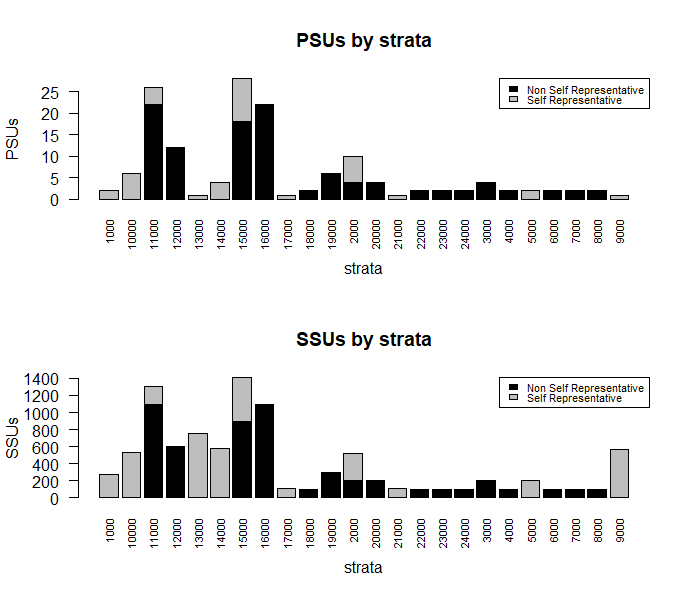
\includegraphics[width=15cm,height=12cm]{allocation2.png}
	\caption{Allocation of PSUs and SSUs (scenario 2).}
	\label{alloca2}
\end{figure}

\subsubsection{Step 5: verify the compliance to precision constraints}

As in the previous scenario, the final check consists in verifying the compliance of the optimized design to the precision constraints.

We, therefore, apply the function \textbf{eval\_2stage}, first for the national level:

\begin{verbatim}
	> # Domain level = national
	> domain_var <- "one"
	> eval21 <- eval_2stage(df,
	+                     PSU_code,
	+                     SSU_code,
	+                     domain_var,
	+                     target_vars,
	+                     PSU_sampled=sample_1st$sample_PSU,
	+                     nsampl=100) 
	> eval21$coeff_var
     CV1    CV2    CV3    CV4  dom
1 0.0102 0.0095 0.0232 0.0354 DOM1
\end{verbatim}
then, at regional level:

\begin{verbatim}
	> # Domain level = regional
	> domain_var <- "region"
	> eval22 <- eval_2stage(df,
	+                     PSU_code,
	+                     SSU_code,
	+                     domain_var,
	+                     target_vars,
	+                     PSU_sampled=sample_1st$sample_PSU,
	+                     nsampl=100) 
	> eval22$coeff_var
     CV1    CV2    CV3    CV4  dom
1 0.0108 0.0067 0.0243 0.0824 DOM1
2 0.0240 0.0202 0.0514 0.0671 DOM2
3 0.0275 0.0353 0.0633 0.0417 DOM3
\end{verbatim}

In this case, the expected precision is slightly higher than the precision constraints in two cases: the fourth variable in domain 1, and the third variable in domain 3. This can be due to the fact that in this scenario the variance of the target variables in strata (on the basis of which the total sample size and the allocation are determined) is not derived from the sampling frame (as in scenario 1), but estimated from a previous round of the survey. 

\section{Comparison with other software}

To evaluate the performance of R2BEAT, in this section we compare it to the other two R packages, i.e.:
\begin{enumerate}
	\item the package \textbf{PracTools} \citep{practools} implements many of the procedures described in \cite{Valliant:2015}, including those regarding the design of multistage samples;
	\item the package \textbf{samplesize4surveys} \citep{Rojas:2020} allows to calculate the sample size for complex surveys.
\end{enumerate}
First, we briefly illustrate, for both packages, the functions covering the two-stage sampling design, then we apply them to the same case seen in scenario 1, finally comparing the obtained results
\footnote{In order to reproduce the processing related to the evaluation of the different software, datasets and R scripts are downloadable from the link  \href{https://zenodo.org/records/10184220}{https://zenodo.org/records/10184220}}.

\subsection{R package PracTools}
\cite{Valliant:2015} describe (pages 231-234) a method for the optimal allocation of two-stage sampling when numbers of sample PSUs and elements per PSU are adjustable (which is our case).

This method is implemented in the R function \textbf{clusOpt2} in the  \textbf{PracTools} package. This function computes the number of PSUs and the number of final units for each PSU for a two-stage sample which uses \textit{srs} at each stage or probability proportional to size with replacement (\textit{ppswr}) at the first stage and \textit{srs} at the second.

This function requires the indication of a number of parameters, among which:
\begin{itemize}
	\item C1: unit cost per PSU
	\item C2: unit cost per SSU
	\item delta: homogeneity measure 
	\item unit.rv: unit relvariance
	\item k: ratio of B2+W2 to unit relvariance
	\item CV0: target CV
	\item tot.cost: total budget for variable costs
	\item cal.sw: indicates if the optimization has to be run for a fixed total budget, or for the target CV0
\end{itemize}

The function \textbf{BW2stagePPS} computes the population values of B2, W2, and delta whose meaning is explained in \cite{Valliant:2015} (page 222).

The method is univariate: the optimization can be performed by indicating only one variable. The whole code required for the case described in scenario 1 is given here:

\begin{verbatim}
	> load("pop.RData")
	> library(PracTools)
	> # Probabilities of inclusion (I stage)
	> pp <- as.numeric(table(pop$municipality))/nrow(pop)
	> # variable income_hh
	> bw <- BW2stagePPS(pop$income_hh, pp, psuID=pop$municipality)
	> bw
	        B2          W2 unit relvar       B2+W2           k       delta 
	0.04075893  0.79538674  0.83601766  0.83614567  1.00015312  0.04874621 
	> des <- clusOpt2(C1=130,
	+                 C2=1,
	+                 delta=bw[6],
	+                 unit.rv=bw[3],
	+                 k=bw[5],
	+                 CV0=0.02,
	+                 tot.cost=NULL,
	+                 cal.sw=2)
	> des
	C1 = 130
	C2 = 1
	delta = 0.04874621
	unit relvar = 0.8360177
	k = 1.000153
	cost = 25499.72
	m.opt = 141.4
	n.opt = 50.4
	CV = 0.02
	> sample_size <- des$m.opt*des$n.opt
	> sample_size
	7126.56 
\end{verbatim}

In running the function, we have indicated that the optimization step was to be carried out having a target CV of 2\% for the variable \textbf{income\_hh}. As there is no way to directly indicate a desired minimum number of SSUs per PSU, we managed to obtain the desired value of 50 by indicating a couple of values 130 and 1 respectively for C1 and C2. As a result, the number of PSUs is 141 and the number of SSUs is 7,127.

\subsection{R package samplesize4surveys}

This package offers two functions to compute a grid of possible sample sizes for estimating single means (\textbf{ss2s4m}) or single proportions (\textbf{ss2s4p}) under two-stage sampling designs.

The required parameters are the following:

\begin{itemize}
	\item N: the population size
	\item mu: the value of the estimated mean of a variable of interest
	\item sigma: the value of the estimated standard deviation of a variable of interest
	\item conf: the statistical confidence
	\item delta: the maximum relative margin of error that can be allowed for the estimation
	\item M: number of clusters in the population
	\item to: (integer) maximum number of final units to be selected per cluster
	\item rho: the intraclass correlation coefficient
\end{itemize}

Here is the code we used in the case of the target variable \textbf{income\_hh}:

\begin{verbatim}
	> load("pop.RData")
	> PSU <- length(unique(pop$municipality))
	> pop_strata <- as.numeric(table(pop$stratum))
	> rho <- 0.04875369 # value taken from scenario 1 analysis
	> ss2s4m(N = nrow(pop), 
	+        mu = mean(pop$income_hh), 
	+        sigma = sd(pop$income_hh),
	+        delta = 0.02 * 1.96, 
	+        M = PSU, 
	+        to = 50, 
	+        rho = sum(rho$RHO_NAR1*pop_strata) / sum(pop_strata))
	50 3.388931 142 50 7061
\end{verbatim}

we obtain a design characterized by a total sample size of 7,061, with 142 PSUs.

Concerning the way we indicated the value of the parameter \textbf{rho}, we made use of the value of the intra-class correlation coefficient computed in scenario 1 by \textbf{R2BEAT}, not considering domains and strata. 

In order to compare the 2\% precision constraint expressed in terms of coefficient of variation, as the package requires the margin of error, we multiply the value of the CV by a z-value equal to 1.96, to obtain the ratio between the semi-width of the confidence interval and the estimate of the mean of the parameter. 

The use of the function \textbf{ss2s4p}, applicable for the other three variables, is practically the same.

\subsection{Comparison of results}
We refer to the scenario 1 setting. 

We consider the same precision levels for the four variables for the unique domain, set respectively to 2\%, 3\%, 3\% and 5\%.

We apply another constraint for all three packages, that is, we want to select a minimum number of final units in each PSU, set to 50. 

There is no problem in doing that for package \textbf{samplesize4surveys}, by setting the parameter \textbf{to} equal to 50: the last value of the final grid is the result we want. Moreover, there is no loss in the optimality of the solution in doing that, because the sample sizes obtained for further values are increasingly higher.

As for \textbf{PractTools}, it is more complicated because there is no direct way to set this constraint. In any case, we manage to do that, by varying the value of C1 (leaving C2 equal to 1) until we find the solution with the nearest value of \textbf{n.opt} to 50.

A final consideration regarding the application of \textbf{R2BEAT}: in this setting, to be comparable with the other packages (that are univariate and mono-domain), it has been applied in a simplified way, that is, one variable per time (univariate), and no different domains and strata in the sampling frame. By so doing, \textbf{R2BEAT} yields obviously different results from those seen in scenario 1.
\begin{table}[h!]
	\caption{Two-stage sample design obtained by different packages.}
	\centering
	\begin{tabular}{|l||c|c|c|c|c|c| }
		\hline
		& \multicolumn{2}{c|}{PracTools} & \multicolumn{2}{c|}{R2BEAT} & \multicolumn{2}{c|}{samplesize4surveys} \\
		Variable   & PSUs &          SSUs           & PSUs &               SSUs               & PSUs &         SSUs         \\ \hline
		active     &  49  &          2459           &  37  &               2030               &  49  &         2436         \\
		inactive   &  90  &          4395           &  68  &               4338               &  88  &         4391         \\
		income\_hh & 141  &          7127           &  79  &               5140               & 142  &         7061         \\
		unemployed & 406  &         19956           & 149  &              10884               & 402  &        20058         \\ \hline
	\end{tabular}
	\label{results}
\end{table}	

\begin{figure} [h!]
	\begin{subfigure}
		\centering
		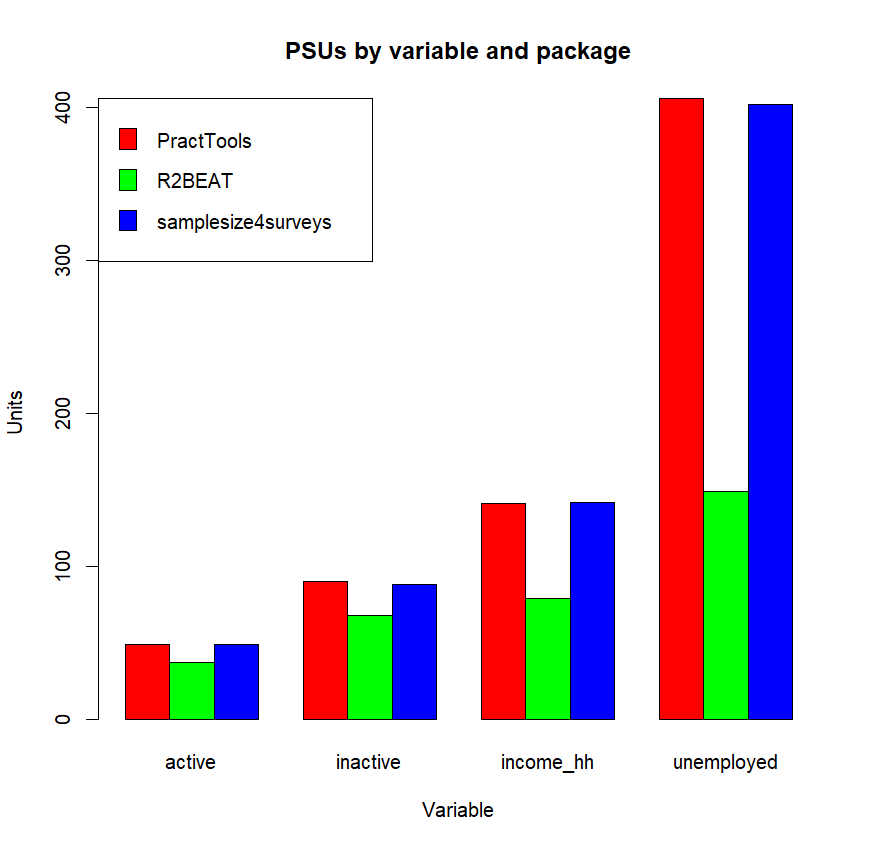
\includegraphics[width=7cm,height=7cm]{comparisonPSU.png}
		\label{comparison:fig1}
	\end{subfigure}
	\begin{subfigure}
		\centering
		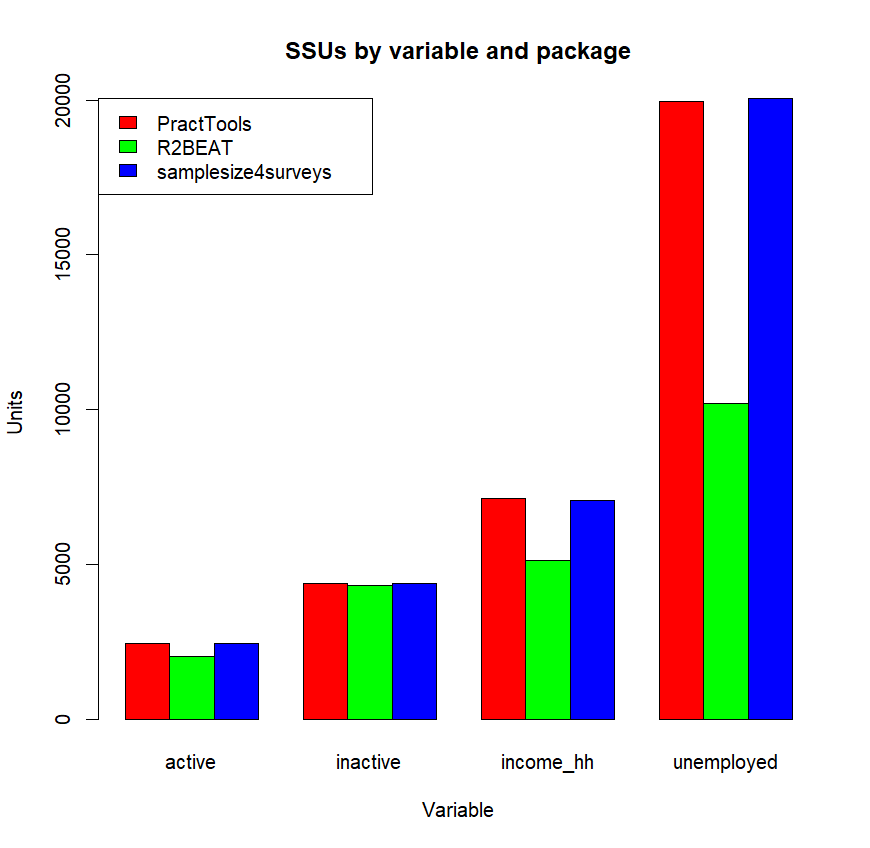
\includegraphics[width=7cm,height=7cm]{comparisonSSU.png}
		\label{comparison:fig2}
	\end{subfigure}
	\caption{Sample sizes by packages.}
	\label{comparison}
\end{figure}

In Table \ref{results} and in Figure \ref{comparison} are reported the results obtained by the three packages.
For checking the reliability of the results, also a simulation has been performed to prove that \textbf{R2BEAT} provides sample sizes that always allow to obtain CVs below the planned ones.

Going in-depth with the comparison among the packages, it can be seen that \textbf{PracTools} and \textbf{samplesize4surveys} have similar behaviors and provide very close results, while \textbf{R2BEAT} always provide samples with smaller sample sizes, both in terms of PSUs and SSUs. 

The differences related to the SSUs are smaller but there are two extremes.
For ``inactive" all three packages yield almost the same results in terms of SSUs, while for ``unemployed” \textbf{R2BEAT} outperforms the other two competitors almost halving their sample sizes.

Juxtaposing Table~\ref{results} and \ref{comparison:cv_rho}, it is possible to see that the differences can be related to the intraclass correlation coefficient, $\rho$.
The differences are maximum in the case of the variable “unemployed” which has the higher $\rho$, and is almost negligible in the case of the variable “inactive” for which $\rho$ is close to 0.

Focusing on the different uses that the three packages make of $\rho$, the differences in the final allocation results arise.
In \textbf{PracTools} and \textbf{samplesize4surveys}, $\rho$ is only involved in the direct calculation of the optimal number of both PSUs and SSUs, once and for all.
Furthermore, in \textbf{samplesize4surveys}, $\rho$ is used only to calculate the $deff$, in turn, used to inflate the variance of the estimate but, also in this case, once and for all.
While, in \textbf{R2BEAT}, $\rho$ is involved in the partition of the PSUs in self-representative (SR) and non-self-representative (NSR). 

This partition, updated every iteration, takes $\rho$  into account each time. In fact, the iterative procedure - and of course the use of $\rho$ in each iteration - makes the results more stable and explores, among all the suitable solutions, the more efficient in terms of PSUs and SSUs.

Summarising, the higher the value of the $\rho$, the higher the efficiency of the R2BEAT algorithm that makes extensive use of the $\rho$ values.

\begin{table}[h!]
	\caption{Intraclass correlation coefficient ($\rho$) for active, inactive, income, and unemployed in the whole population.}
	\centering
	\begin{tabular}{|l||c|}
		\hline
		Variable    & $\rho$ \\ 
            \hline
		active      & 0.0656 \\ 
            inactive    & 0.0021 \\
		income\_hh  & 0.0488 \\ 
            unemployed  & 0.1263. 
            \\
            \hline
	\end{tabular}
	\label{comparison:cv_rho}
\end{table}	




\section{How to manage the total non-response}
Sample size and allocation in strata provided by \textbf{R2BEAT} ensure compliance with the precision constraints. 
Unfortunately, in practice, the planned sample size is affected by total non-response which reduces it and, consequently, weakens the precision and efficiency of the estimates.
Therefore, it is important to consider the total non-response when planning sample surveys and to implement strategies to preserve the precision of the estimates. 

%The sample size, both PSUs and SSUs to be selected, should always consider that, unfortunately, not all the selected sampled statistical units will participate in the survey, answering the questionnaire. 
%Total non-response is a common issue in sample surveys (even in mandatory ones, or in the census) that lead to a reduction in the sample size and an increase in non-response bias. 
%To consider total non-response in designing a sample survey, it is important to consider into the sample some other units, which will be sampled in case of non-response of some units else. 

The most common methods to carry out this task at the planning stage are \textit{oversampling} and \textit{substitutions}. 

Oversampling is a technique used to increase the sample size of a population in a survey according to the total non-response rate in the population strata ($nrr_h$, with $0\leq nrr_h \leq 1$ and $h=1,\dots,H$) for recovering, at the end of the data collection phase, the desired sample size and the expected precision requirements.
These rates are usually derived from previous survey occasions, carried out with the same data collection technique and under similar conditions, or on reliable assumptions made by those who design the survey. 
For embedding this procedure in \textbf{R2BEAT}, before performing the selection of the SSUs, it is sufficient to multiply the column \textbf{PSU\_final\_sample\_unit} of the \textbf{data.frame} \textbf{sample\_PSU} provided as the output of the function \textbf{select\_PSU} by $1+nrr_h$. 
If the response rates are not available at the strata level but at a higher domain level (for instance, for domains that are aggregations of strata), it is possible to assume a constant non-response rate for the strata belonging to the same domain.
Of course, the more precise the knowledge of response rates, the more accurate the oversampling procedure adopted will be. 

Instead, substitutions involve replacing non-responding units with other ones which have been ``a priori" selected.
Sometimes even more than one substitute for a single SSU is singled out.
The selection of substitute units can be carried out in different ways \citep[see, for a brief but complete review][]{lynn2004use}. 
If a simple random substitution of the SSUs, before performing the selection of the SSU, it is sufficient to multiply the column \textbf{PSU\_final\_sample\_unit} of the \textbf{data.frame} \textbf{sample\_PSU} provided as the output of the function \textbf{select\_PSU} by the chosen number of substitutes. 
Otherwise, if a non-random substitution or a stratified substitution, unlike in the previous case, the selection of SSUs requires additional information on the SSUs and, therefore, the use of ad hoc solutions. 

However, it is important to point out that substitutions and oversampling aim to preserve the sample size inflating it to withstand the non-response. 
However, it could be anyway not enough to avoid total non-response bias side effects on the final estimates.
Therefore, non-response treatment methods must be applied after the data collection phase \citep[see, e.g.,][]{sarndal2005estimation, little2019statistical}.



\section{Concluding remarks}
Methodology, completeness, and efficiency can be considered the main strengths of the R package R2BEAT. 

The methodology based on the application of the Bethel algorithm ensures that the resulting sample designs
are compliant with the precision constraints set on the target estimates of a given survey.

The completeness can be considered both:
\begin{itemize}
	\item in terms of applicability: R2BEAT applies to stratified, multipurpose and multidomain, one-stage and
two-stage sampling surveys;
	\item in terms of coverage of the user needs: the package covers all the steps of a complex sample design, 
from the setting of precision constraints, the determination of the total sample size and of the allocation in the strata and the selection of the sampling units, distinctly according to the stage of selection.
\end{itemize}
Moreover, a set of functions generates the input required by the optimization step starting from the availability of a sampling frame and/or a previous round of the survey, thus allowing 
the users to fully harness all the available information with minimal effort. Other functions help them to perform analysis and checks on the obtained allocations and the selected sample.

Finally, we demonstrated the efficiency of the package by comparing it with two other competitor packages in terms of the results obtained in a case study: on equal errors, the sample size determined by R2BEAT is always lower,
in terms of both Primary and Secondary Stage Units (PSUs and SSUs).

In future work, considering that a limitation of the package is its applicability to only mean parameters, the
extension to more complex parameters will be investigated.




\hypertarget{refs}{}

\bibliography{RJreferences.bib}

\address{%
Giulio Barcaroli\\
Independent consultant\\%
via Monte delle Gioie 29 - 00199 Roma\\ Italy\\
%
%
%
\href{mailto:gbarcaroli@gmail.com}{\nolinkurl{gbarcaroli@gmail.com}}%
}

\address{%
Andrea Fasulo\\
Italian National Institute of Statistics\\%
via Cesare Balbo 16 - 00184 Roma\\ Italy\\
%
%
%
\href{mailto:andrea.fasulo@istat.it}{\nolinkurl{andrea.fasulo@istat.it}}%
}

\address{%
Alessio Guandalini\\
Italian National Institute of Statistics\\%
via Cesare Balbo 16 - 00184 Roma\\ Italy\\
%
%
%
\href{mailto:alessio.guandalini@istat.it}{\nolinkurl{alessio.guandalini@istat.it}}%
}

\address{%
Marco D. Terribili\\
Italian National Institute of Statistics\\%
via Cesare Balbo 16 - 00184 Roma\\ Italy\\
%
%
%
\href{mailto:marco.terribili@istat.it}{\nolinkurl{marco.terribili@istat.it}}%
}

\end{article}


\end{document}
